%# -*- coding: utf-8-unix -*-
%%==================================================

\chapter{AVL and BST}
\label{chap7}

\begin{itemize}[noitemsep,topsep=0pt,parsep=0pt,partopsep=0pt]
	\item 知识点:讲解相关知识点。
	\item 题型:直接上真题。
\end{itemize}

\section{知识点和方法论}

\subsection{知识点}
\begin{itemize}[noitemsep,topsep=0pt,parsep=0pt,partopsep=0pt]
	\item 二叉平衡树 BST, 所有$\mbox{左孩子} \le \mbox{根结点} \le \mbox{右孩子}$
	\item 二叉排序树 AVL,也是一棵BST树,也满足BST的相关性质。
	\begin{itemize}[noitemsep,topsep=0pt,parsep=0pt,partopsep=0pt]
		\item 平衡因子的计算 $ \mbox{平衡因子} = \mbox{左子树的高度} - \mbox{右子树的高度} $
		\item 以平衡因子绝对值大于1的节点作为根节点
	\end{itemize}
\end{itemize}

\subsection{方法论}
\begin{itemize}[noitemsep,topsep=0pt,parsep=0pt,partopsep=0pt]
	\item 平衡二叉树的插入节点方法
	\begin{itemize}[noitemsep,topsep=0pt,parsep=0pt,partopsep=0pt]
		\item 圈出三个不平衡的节点,然后按照 小 中 大 的顺序,重新排列即可.可能还要移动一些元素配合移动。{\color{red}靠近最大不平衡的三个节点}.
		\item LL平衡旋转({\color{red}右单旋转}),由于在节点A的左孩子({\color{red}L})的左子树({\color{red}L})上插入了新结点,A失去平衡。向右转一下,即可。
		\item RR平衡旋转({\color{red}左单旋转}),由于在节点A的右孩子(R)的右子树(R)上插入了新节点,A的平衡因子由-1减至-2,导致以A为根的子树失去平衡,需要一次向左的旋转操作。
		\item LR平衡旋转(先左后右双旋转)。由于在A的左孩子(L)的右子树(R)上插入新结点,A的平衡因子由1增至2,导致以A为根的子树失去平衡,需要进行两次旋转操作,先左旋后右旋。
		\item RL 平衡旋转(先右后左双旋转)。由于在A的右孩子(R)的左子树(L)上插入新结点,A的平衡因子由-1减至-2,导致以A为根的子树失去平衡,先右旋,再左旋。
		\item 参考视频连接 \url{https://www.bilibili.com/video/av14273075/?p=2}
	\end{itemize}
\end{itemize}

\section{真题实战}


\subsection{2017年第5题}

\begin{lstlisting}[basicstyle=\small\ttfamily, caption={}, numbers=none]
5. 设数据元素的关键字序列为(20,30,15,45,78,65,25,60)依次插入这些元素,创建一颗平衡的二叉排序树(AVL树),请逐一画出每插入一个元素后的AVL
树的形态。
\end{lstlisting}
解:\newline
\begin{figure}[H]
	\centering  % 环境中的内容居中排版
	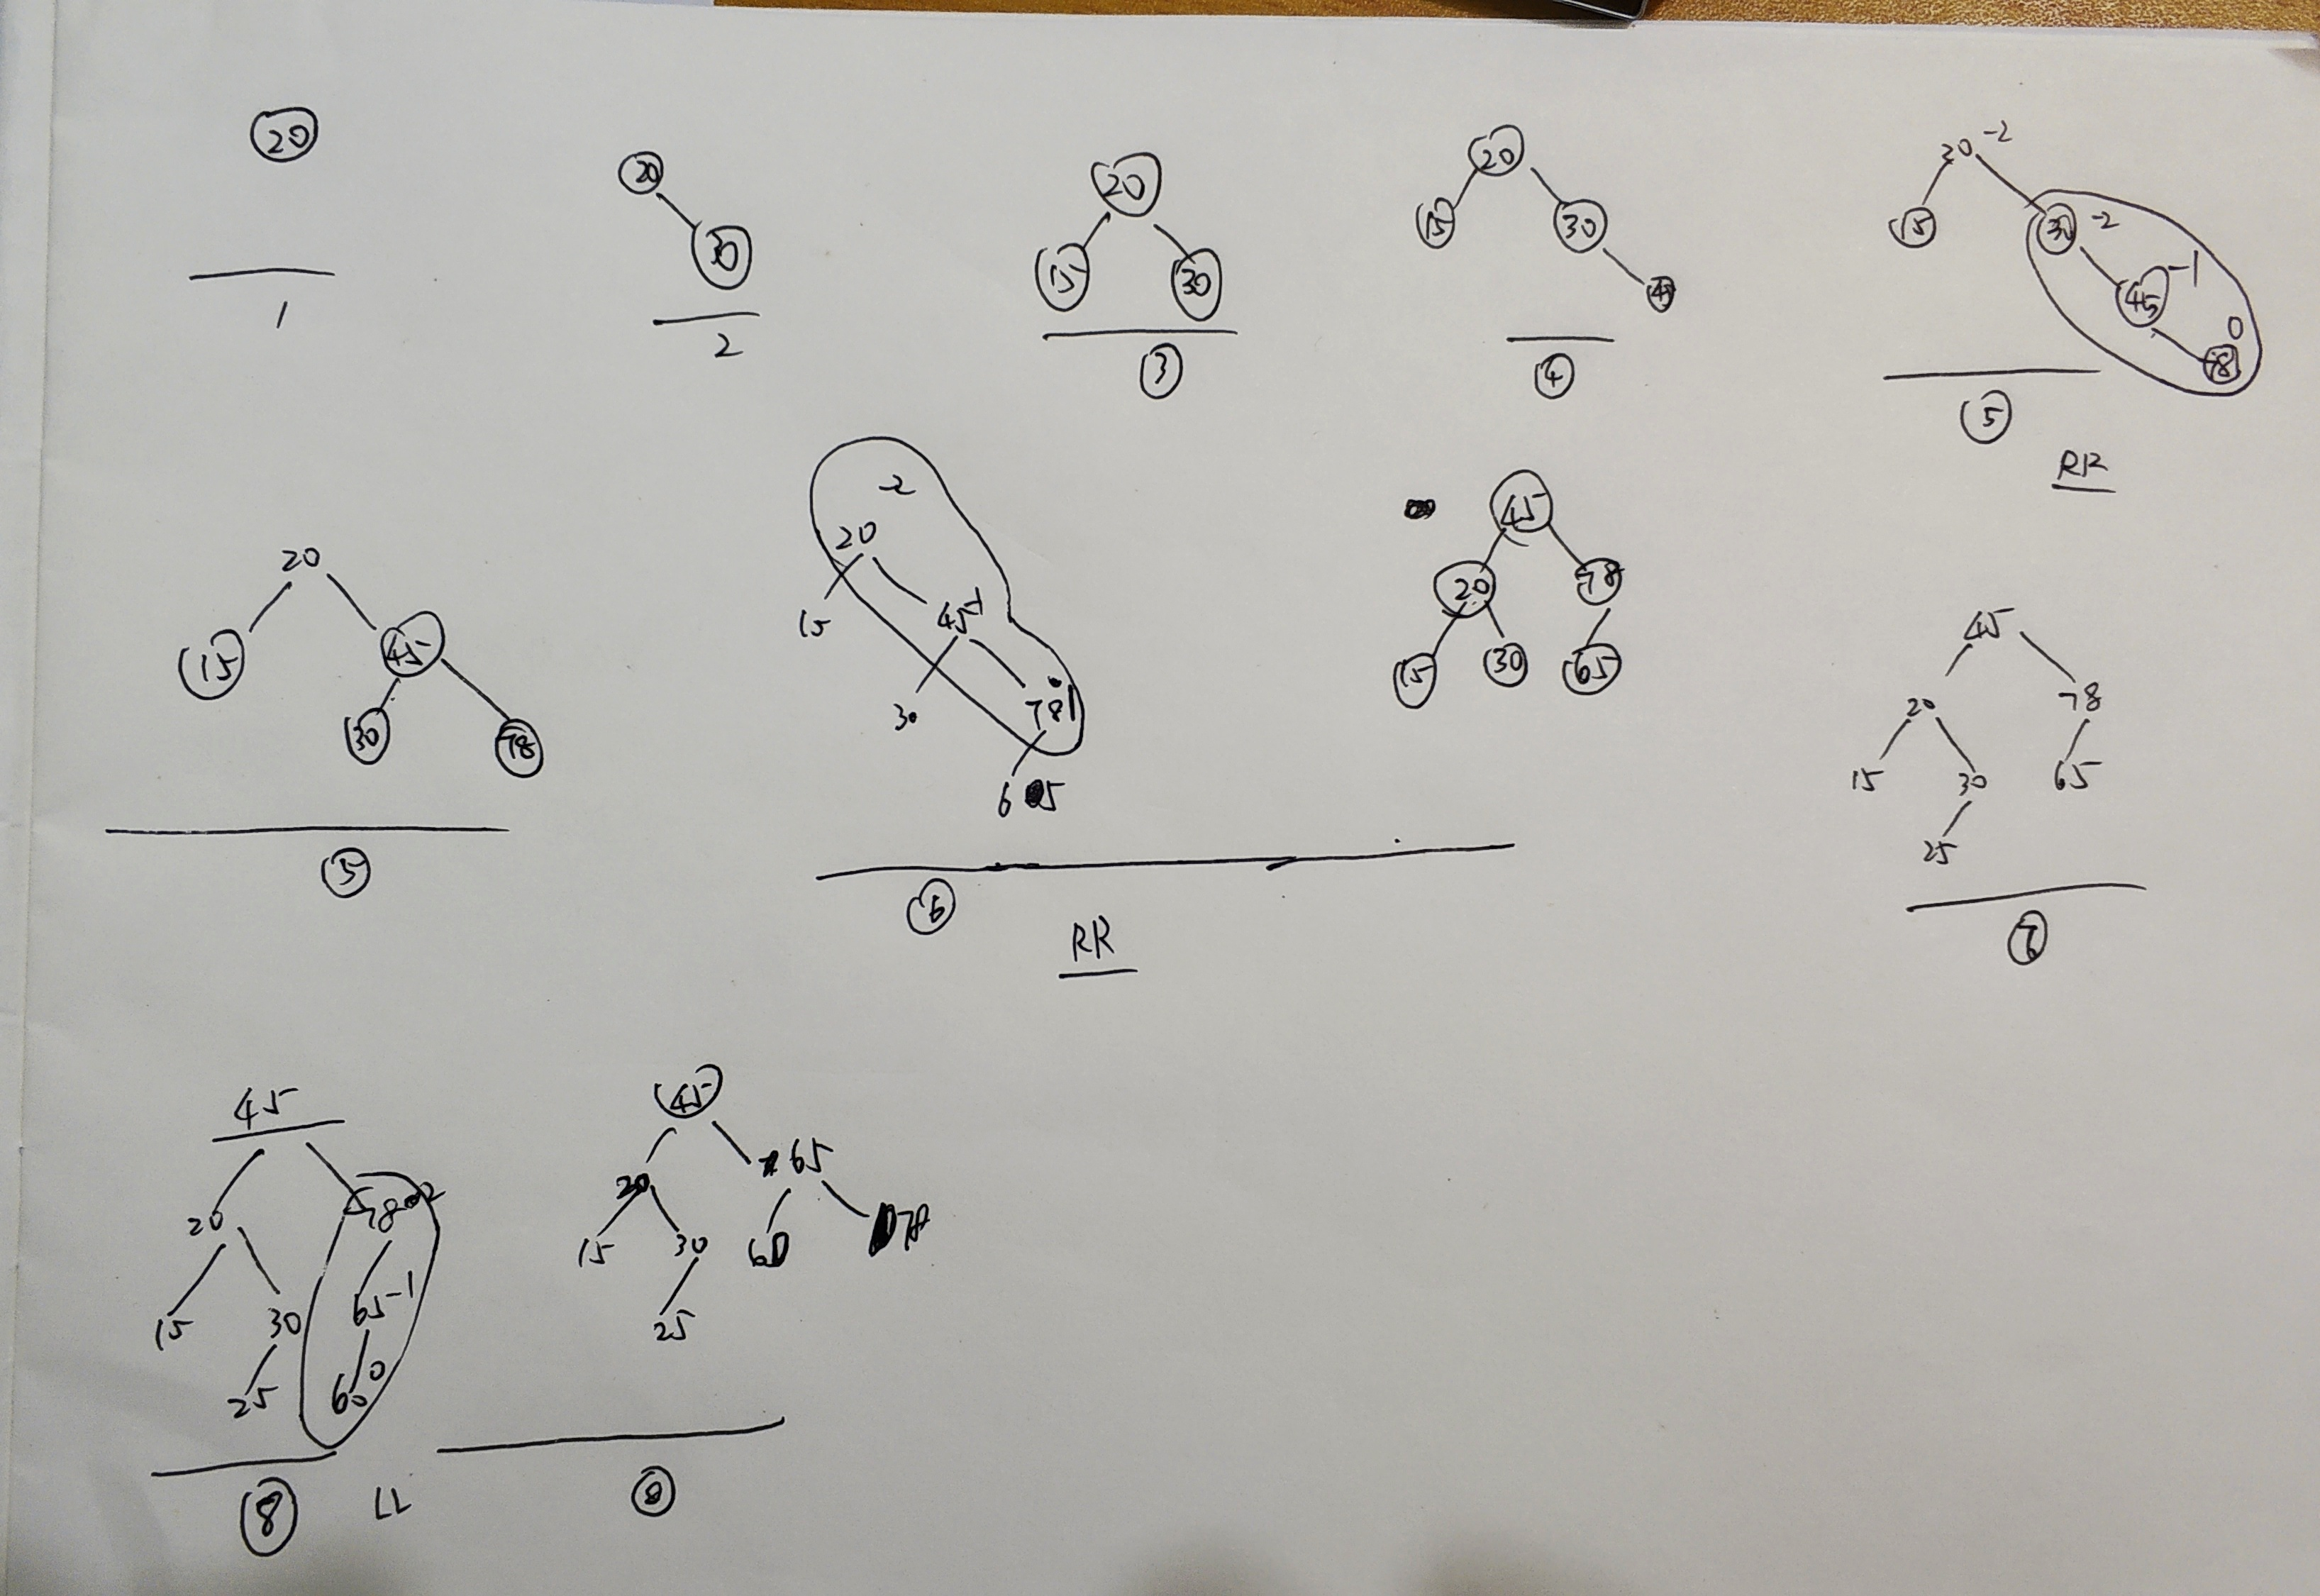
\includegraphics[scale=0.1]{example/chapter7/2018-12-03_16-40-08_366.png}
\end{figure}

\subsection{2010年408}
在如题图所示的平衡二叉树中插入关键字48后得到一棵新平衡二叉树,在新平衡二叉树中,关键字37所在节点的左、右子节点中保存的关键字分别是(   )\newline
A. 13,48    B.24,48  C. 24,53   D. 24, 90\newline
\begin{figure}[H]
	\centering  % 环境中的内容居中排版
	\includegraphics[scale=0.1]{example/chapter7/Annotation2019-09-24152618.png}
\end{figure}
解:\newline
\begin{figure}[H]
	\centering  % 环境中的内容居中排版
	\includegraphics[scale=0.1]{example/chapter7/QQ20190923230023.jpg}
\end{figure}

\subsection{2013年408}
若将关键字1,2,3,4,5,6,7依次插入的初始为空的平衡二叉树T中,则T中平衡因子为0的分支节点的个数是(   )\newline
A. 0   B. 1  C. 2  D. 3
解:\newline
D.3个。
\begin{figure}[H]
	\centering  % 环境中的内容居中排版
	\includegraphics[scale=0.1]{example/chapter7/QQ20190924154030.jpg}
\end{figure}




